\newcommand{\fileInfectorTagResultsAucTable}{
    \begin{table}[H]
        \centering
        \begin{tabular}{|p{2,8cm}||P{2,2cm} P{2,2cm} P{2,2cm} P{2,2cm}|}
            \hline
            File-infector Tag & ALOHA\newline (M/B only) & ALOHA & Joint\newline Embedding & Proposed\newline Model \\
            \hline
            AUC-ROC & - & 0.985$\pm$0.000 & 0.986$\pm$0.000 & \textBF{0.987$\pm$0.002} \\
            \hline
        \end{tabular}
        \caption[File-infector Tag prediction task AUC-ROC results]{AUC-ROC (Area Under Curve) of the different models for the \textbf{File-infector Tag} prediction task. Results were aggregated over \textBF{3} training runs with different weight initializations and minibatch orderings. Best results are shown in \textbf{bold}.} \label{tab:fileInfectorTag_auc}
    \end{table}
}

\newcommand{\fileInfectorTagResultsAtFprTable}{
    \begin{center}
        \begin{longtable}[c]{|P{3,2cm}||P{1,8cm} P{1,8cm} P{1,8cm} P{1,8cm} P{1,8cm}|}
            \hline
            File-infector Tag & \multicolumn{5}{c|}{{FPR}} \\
            & $10^{-5}$ & $10^{-4}$ & $10^{-3}$ & $10^{-2}$ & $10^{-1}$ \\
            \hline
            \endfirsthead

            \caption*{\raggedright ...continued from previous page} \\
            \hline
            File-infector Tag & \multicolumn{5}{c|}{\textbf{FPR}} \\
            & $10^{-5}$ & $10^{-4}$ & $10^{-3}$ & $10^{-2}$ & $10^{-1}$ \\
            \hline
            \endhead

            \caption*{\raggedleft ...continued on next page} \\
            \endfoot

            \caption[File-infector Tag prediction task results]{Mean and standard deviation results (TPR, Accuracy, Recall, Precision and F1-Score) of the different models for the \textbf{File-infector Tag} prediction task at different \textbf{FPR}s (\textit{False Positive Rates}). Results were aggregated over \textBF{3} training runs with different weight initializations and minibatch orderings. Best results are shown in \textbf{bold}. Under \textbf{TPR} results are also presented the percentage reduction in mean detection error and in ROC curve standard deviation introduced by the \textit{Proposed Model} with respect to both \textit{ALOHA} model and \textit{Joint Embedding}.} \label{tab:fileInfectorTag_results_at_fpr} \\
            \endlastfoot

            \multicolumn{6}{|c|}{\textbf{TPR}} \\
            \hline
            ALOHA (M/B only) & - & - & - & - & - \\
            ALOHA & 0.263$\pm$0.110 & 0.419$\pm$0.081 & 0.821$\pm$0.013 & 0.875$\pm$0.003 & 0.953$\pm$0.001 \\
            Joint Embedding & \textBF{0.500$\pm$0.133} & \textBF{0.681$\pm$0.084} & 0.822$\pm$0.041 & 0.867$\pm$0.015 & \textBF{0.962$\pm$0.003} \\
            Proposed Model & 0.275$\pm$0.263 & 0.449$\pm$0.246 & \textBF{0.850$\pm$0.016} & \textBF{0.883$\pm$0.014} & 0.959$\pm$0.012 \\
            \hline
            Error Reduction wrt\newline ALOHA (M/B only) & - & - & - & - & - \\
            Error Reduction wrt\newline ALOHA & 1.6\% & 5.2\% & 16.2\% & 6.4\% & 12.8\% \\
            Error Reduction wrt\newline Joint Embedding & -45.0\% & -72.7\% & 15.7\% & 12.0\% & -7.9\% \\
            \hline
            Std Reduction wrt\newline ALOHA (M/B only) & - & - & - & - & - \\
            Std Reduction wrt\newline ALOHA & -139.1\% & -203.7\% & -23.1\% & -366.7\% & -1100.0\% \\
            Std Reduction wrt\newline Joint Embedding & -97.7\% & -192.9\% & 61.0\% & 6.7\% & -300.0\% \\
            \hline
            \multicolumn{6}{|c|}{\textbf{Accuracy}} \\
            \hline
            ALOHA (M/B only) & - & - & - & - & - \\
            ALOHA & 0.881$\pm$0.018 & 0.906$\pm$0.013 & 0.970$\pm$0.002 & 0.971$\pm$0.001 & 0.908$\pm$0.000 \\
            Joint Embedding & \textBF{0.919$\pm$0.021} & \textBF{0.948$\pm$0.014} & 0.970$\pm$0.007 & 0.970$\pm$0.002 & \textBF{0.910$\pm$0.001} \\
            Proposed Model & 0.883$\pm$0.043 & 0.911$\pm$0.040 & \textBF{0.975$\pm$0.003} & \textBF{0.973$\pm$0.002} & 0.910$\pm$0.002 \\
            \hline
            \multicolumn{6}{|c|}{\textbf{Recall}} \\
            \hline
            ALOHA (M/B only) & - & - & - & - & - \\
            ALOHA & 0.263$\pm$0.110 & 0.419$\pm$0.081 & 0.821$\pm$0.013 & 0.875$\pm$0.003 & 0.953$\pm$0.001 \\
            Joint Embedding & \textBF{0.500$\pm$0.133} & \textBF{0.681$\pm$0.084} & 0.822$\pm$0.041 & 0.867$\pm$0.015 & \textBF{0.962$\pm$0.003} \\
            Proposed Model & 0.275$\pm$0.264 & 0.448$\pm$0.247 & \textBF{0.850$\pm$0.016} & \textBF{0.883$\pm$0.014} & 0.959$\pm$0.012 \\
            \hline
            \multicolumn{6}{|c|}{\textbf{Precision}} \\
            \hline
            ALOHA (M/B only) & - & - & - & - & - \\
            ALOHA & \textBF{1.000$\pm$0.000} & \textBF{0.999$\pm$0.000} & \textBF{0.994$\pm$0.000} & 0.944$\pm$0.000 & 0.647$\pm$0.000 \\
            Joint Embedding & \textBF{1.000$\pm$0.000} & \textBF{0.999$\pm$0.000} & \textBF{0.994$\pm$0.000} & 0.943$\pm$0.001 & \textBF{0.650$\pm$0.001} \\
            Proposed Model & 0.999$\pm$0.001 & 0.999$\pm$0.001 & \textBF{0.994$\pm$0.000} & \textBF{0.945$\pm$0.001} & 0.649$\pm$0.003 \\
            \hline
            \multicolumn{6}{|c|}{\textbf{F1 Score}} \\
            \hline
            ALOHA (M/B only) & - & - & - & - & - \\
            ALOHA & 0.405$\pm$0.133 & 0.586$\pm$0.082 & 0.899$\pm$0.008 & 0.908$\pm$0.002 & 0.771$\pm$0.001 \\
            Joint Embedding & \textBF{0.656$\pm$0.112} & \textBF{0.807$\pm$0.060} & 0.899$\pm$0.025 & 0.903$\pm$0.009 & \textBF{0.775$\pm$0.002} \\
            Proposed Model & 0.369$\pm$0.302 & 0.582$\pm$0.218 & \textBF{0.916$\pm$0.009} & \textBF{0.913$\pm$0.008} & 0.774$\pm$0.006 \\
            \hline
        \end{longtable}
    \end{center}
}

\newcommand{\fileInfectorTagResultsSummaryTable}{
    \begin{table}[H]
        \centering
        \begin{tabular}{|P{3,2cm}||P{1,8cm} P{1,8cm} P{1,8cm} P{1,8cm} P{1,8cm}|}
            \hline
            \multicolumn{6}{|c|}{File-infector Tag (at FPR $=1\%$)} \\
            \hline
            Model & TPR & Accuracy & Precision & Recall & F1 score \\
            \hline
            ALOHA (M/B only) & - & - & - & - & - \\
            ALOHA & 0.875$\pm$0.003 & 0.971$\pm$0.001 & 0.944$\pm$0.000 & 0.875$\pm$0.003 & 0.908$\pm$0.002 \\
            Joint Embedding & 0.867$\pm$0.015 & 0.970$\pm$0.002 & 0.943$\pm$0.001 & 0.867$\pm$0.015 & 0.903$\pm$0.009 \\
            Proposed Model & \textBF{0.883$\pm$0.014} & \textBF{0.973$\pm$0.002} & \textBF{0.945$\pm$0.001} & \textBF{0.883$\pm$0.014} & \textBF{0.913$\pm$0.008} \\
            \hline
        \end{tabular}
        \caption[Summary of File-infector Tag prediction task results]{Summary of the mean and standard deviation results of the different models for the \textbf{File-infector Tag} prediction task at \textbf{FPR} $=1\%$. Results were aggregated over \textBF{3} training runs with different weight initializations and minibatch orderings. Best results are shown in \textbf{bold}.} \label{tab:fileInfectorTag_result_summary}
    \end{table}
}

\newcommand{\fileInfectorTagRocAlohaMB}{
    \begin{figure}[H]
        \vspace*{-0.5cm}
        \centering
        \includegraphics[width=0.6\textwidth]{./results/file_infector_tag_roc_alohaMB.png}
        \vspace*{-0.2cm}
        \caption[File-infector Tag prediction task ALOHA (M/B only) ROC curve]{ROC curve and AUC statistics of \textBF{ALOHA (M/B only)} model for the \textbf{File-infector Tag}. The line represents the \textit{mean} TPR at a given FPR, while the shaded region represents the \textit{standard deviation}. Statistics were computed over \textBF{3} training runs, each with random parameter initialization.}
        \label{fig:fileInfectorTagRocAlohaMB}
    \end{figure}
}

\newcommand{\fileInfectorTagRocAloha}{
    \begin{figure}[H]
        \vspace*{-0.5cm}
        \centering
        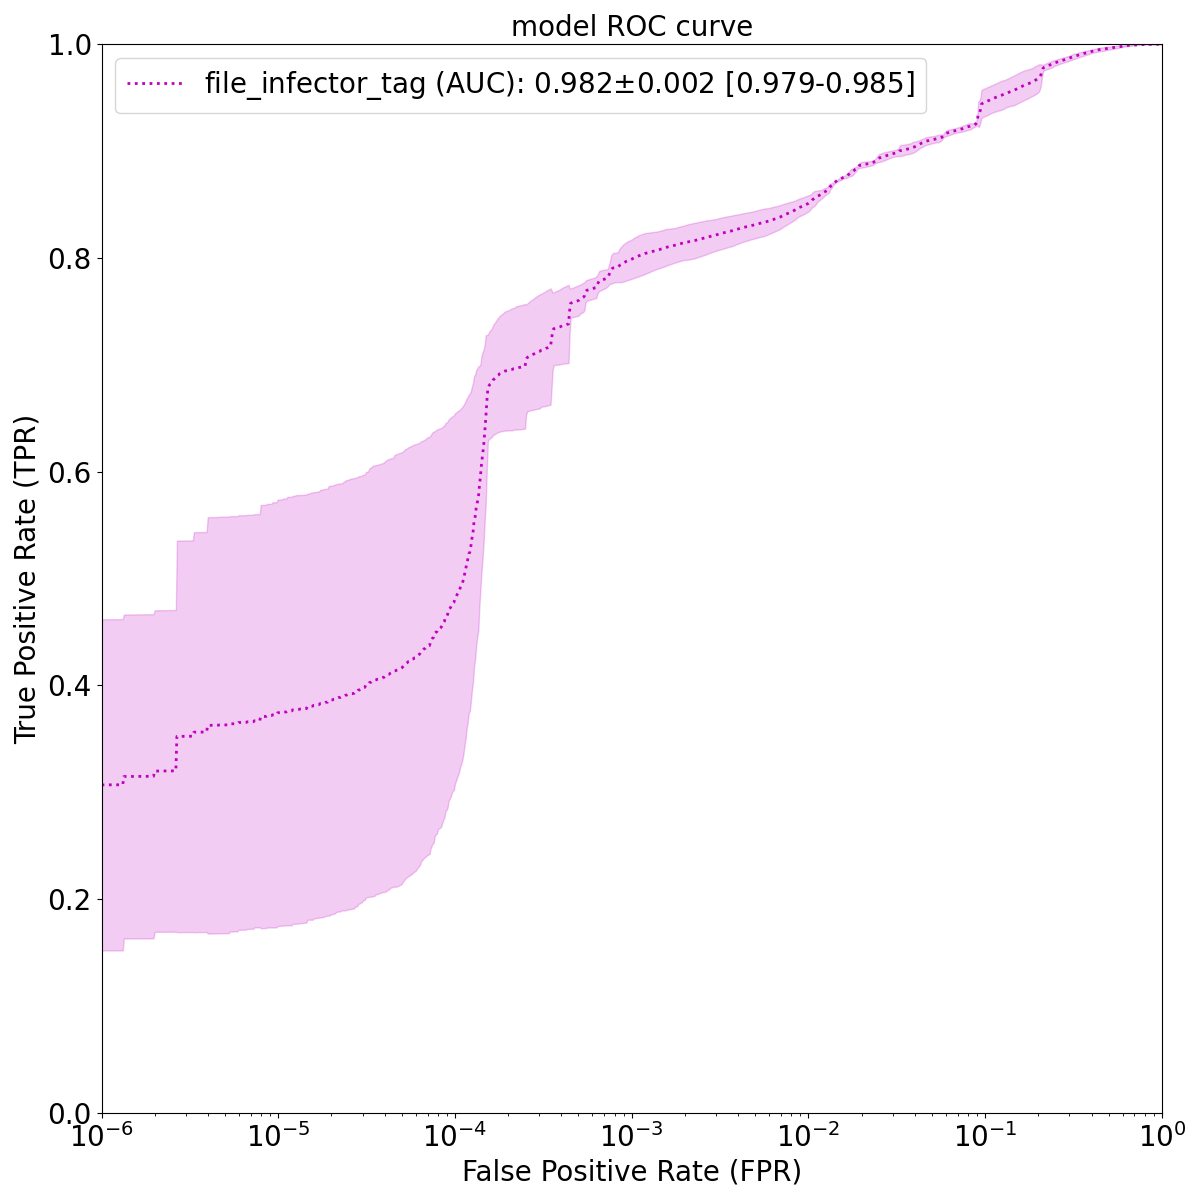
\includegraphics[width=0.6\textwidth]{./results/file_infector_tag_roc_aloha.png}
        \vspace*{-0.2cm}
        \caption[File-infector Tag prediction task ALOHA ROC curve]{ROC curve and AUC statistics of \textBF{ALOHA} model for the \textbf{File-infector Tag}. The line represents the \textit{mean} TPR at a given FPR, while the shaded region represents the \textit{standard deviation}. Statistics were computed over \textBF{3} training runs, each with random parameter initialization.}
        \label{fig:fileInfectorTagRocAloha}
    \end{figure}
}

\newcommand{\fileInfectorTagRocJointEmbedding}{
    \begin{figure}[H]
        \vspace*{-0.5cm}
        \centering
        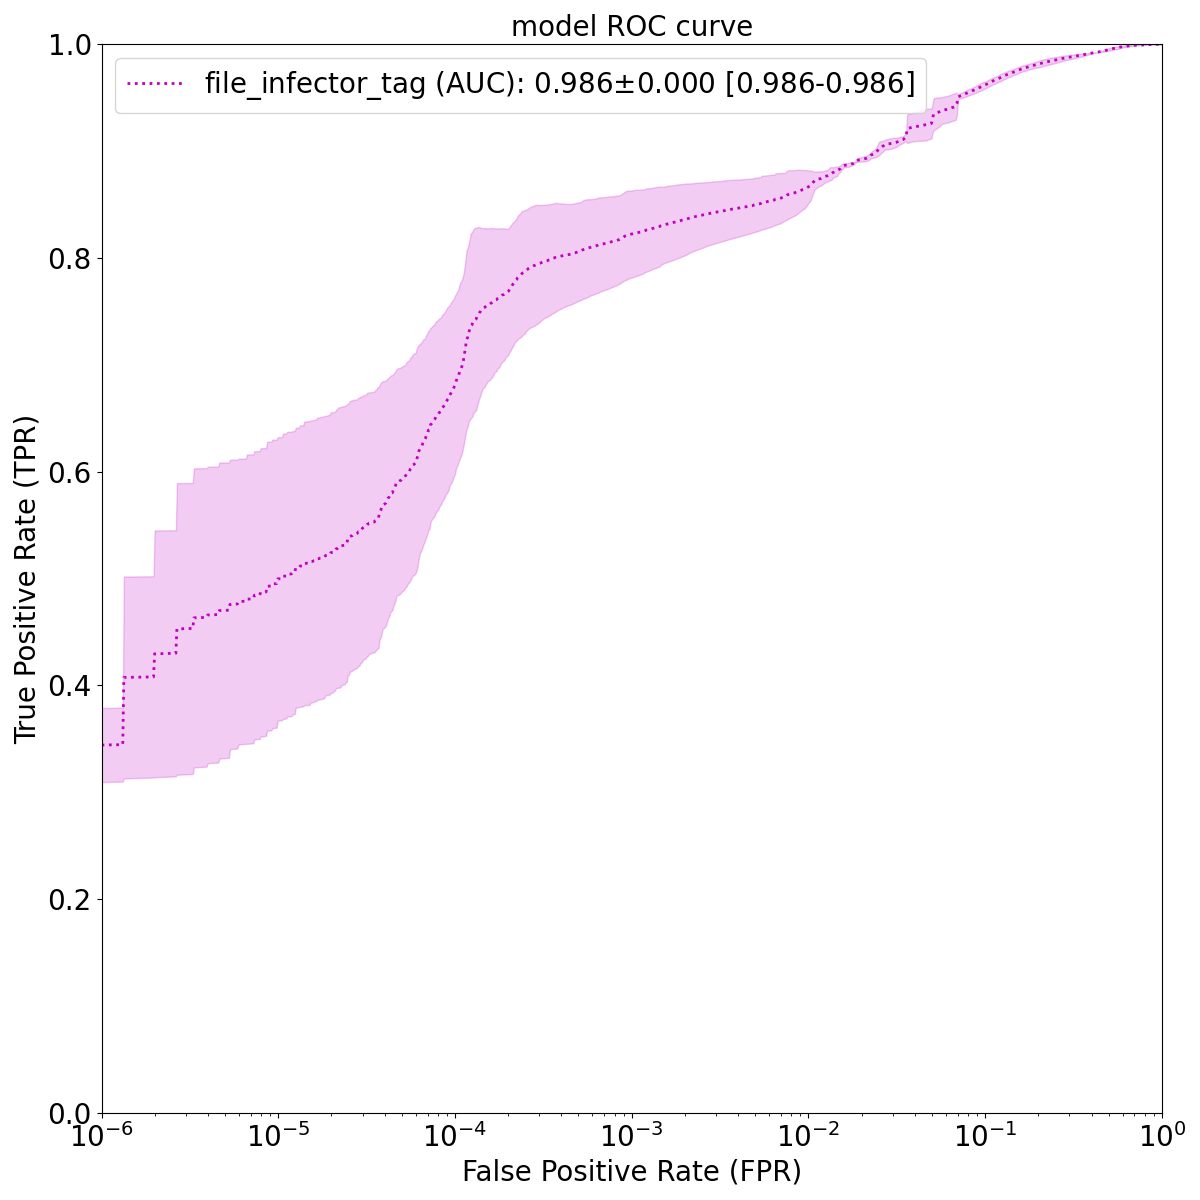
\includegraphics[width=0.6\textwidth]{./results/file_infector_tag_roc_jointEmbedding.png}
        \vspace*{-0.2cm}
        \caption[File-infector Tag prediction task Joint Embedding ROC curve]{ROC curve and AUC statistics of \textBF{Joint Embedding} model for the \textbf{File-infector Tag}. The line represents the \textit{mean} TPR at a given FPR, while the shaded region represents the \textit{standard deviation}. Statistics were computed over \textBF{3} training runs, each with random parameter initialization.}
        \label{fig:fileInfectorTagRocJointEmbedding}
    \end{figure}
}

\newcommand{\fileInfectorTagRocProposedMethod}{
    \begin{figure}[H]
        \vspace*{-0.5cm}
        \centering
        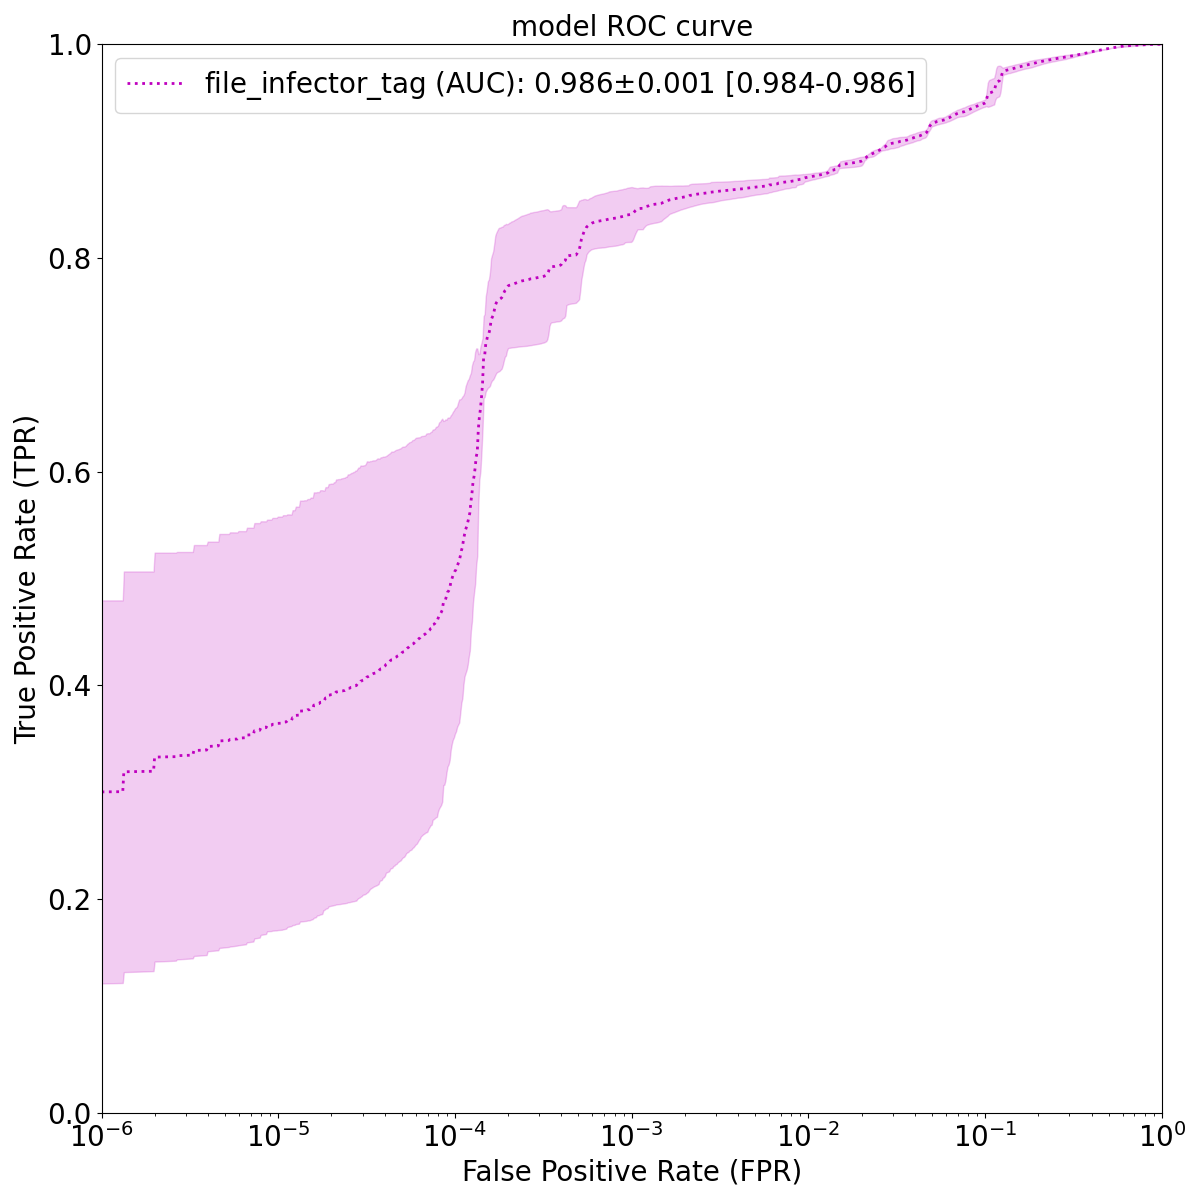
\includegraphics[width=0.6\textwidth]{./results/file_infector_tag_roc_proposedModel.png}
        \vspace*{-0.2cm}
        \caption[File-infector Tag prediction task Proposed Model ROC curve]{ROC curve and AUC statistics of \textBF{Proposed Model} for the \textbf{File-infector Tag}. The line represents the \textit{mean} TPR at a given FPR, while the shaded region represents the \textit{standard deviation}. Statistics were computed over \textBF{3} training runs, each with random parameter initialization.}
        \label{fig:fileInfectorTagRocProposedModel}
    \end{figure}
}
